\documentclass{article}
\usepackage[utf8]{inputenc}

\title{Functional Game Programming}
\author{David Kraeutmann}

\usepackage{natbib}
\usepackage{graphicx}
\usepackage{url}
\usepackage{amsmath}
\usepackage{amssymb}
\usepackage{amsthm}
\usepackage{enumitem}
\usepackage{minted}
\usepackage{parcolumns}
\usepackage[normalem]{ulem}
\usepackage{multicol}
\usepackage{caption}
\usepackage[a4paper]{geometry}

\usepackage{tikz}
\usetikzlibrary{shapes,snakes}
\usetikzlibrary{scopes,backgrounds}

\tikzset{signal function/.style={draw=black, rectangle, minimum width=6em}}
\tikzset{signal function with state/.style={draw=black, rectangle split, rectangle split parts = 2, rectangle split draw splits = false, minimum width=6em}}

\usepackage{fancyvrb}
\DefineShortVerb{\|}

\begin{document}
\maketitle]

\section{Introduction}
Real-time programming is at its core quite imperative --- read input, update state, write output, repeat. 
That requires you to describe \emph{what to do} instead of \emph{what you want}, which leads to a lot of boilerplate when just trying to model a state update.
However, without additional thought even programs written using declarative programming lose their unique benefits due to the imperative style imposed by the update loop, large amounts of state and discrete-time semantics. 
\begin{listing}[ht]
\inputminted[breaklines=true]{haskell}{../vortrag_david/Loop.hs}
\captionof{listing}{Update loop of a Haskell program}
\label{lst:imperative}
\end{listing}

To address these issues, Elliott/Hudak formulated \emph{Functional Reactive Programming} (FRP) in \cite{ElliottHudak97:Fran}. FRP evolved in a myriad of different directions and has  applications in robotics, computer vision, animation and games \cite{haskell-wiki-yampa}. 
We'll provide an overview of FRP \cite{hudak2003arrows} in Section~\ref{sec:frp}
and focus on Netwire and Elm in particular as implementations in Section~\ref{sec:frameworks}.
A small game written in Elm is presented (Section~\ref{sec:game}) and <insert more text here>. 
In (Section~\ref{sec:conclusion}) we provide an overview of benefits and unsolved problems of functional game systems.

\section{Functional reactive programming}
\label{sec:frp}
\subsection{Signal functions}
\begin{figure}[ht]
\centering
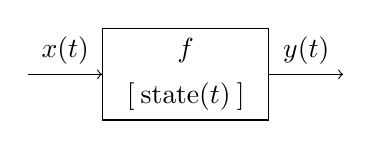
\begin{tikzpicture}[node distance=2cm]
\node[signal function with state] (arrf) {$f$ \nodepart{second} $[\: \operatorname{state}(t) \: ]$};
\coordinate[left of=arrf] (in);
\coordinate[right of=arrf] (out);
\draw [->] (in) to node[auto] {$x(t)$} (arrf);
\draw [->] (arrf) to node[auto] {$y(t)$} (out);
\end{tikzpicture}
\captionof{figure}{Signal function}
\label{fig:sigfunc}
\end{figure}

\section{FRP frameworks}
\label{sec:frameworks}

\section{A functional game}
\label{sec:game}

\section{Related works}
\label{sec:related}
Conal Elliott's paper "Push-pull functional reactive programming" \cite{Elliott2009-push-pull-frp} serves an integral role in modern FRP
and serves as the theoretical basis of many FRP libraries. Alexander Berntsen master thesis on programming game systems in Haskell \cite{Berntsen2014-game-systems-haskell} compares imperative and functional game design based on a medium-sized game and provides substantial evidence supporting the usage of strongly static typed purely functional programming for game development. Charles' post about recreating Asteroids in Netwire \cite{asteroids} describes difficulties encountered when implementing a game using Netwire.
\section{Conclusion and Outlook}
\label{sec:conclusion}

\bibliographystyle{plain}
\bibliography{references}
\end{document}
